
\documentclass[12pt,fleqn]{article}  
\usepackage{amsmath}
\usepackage{amssymb}
\usepackage{graphicx}

\pagestyle{empty}

\unitlength 1cm
\textheight 22cm
\textwidth 17cm
\oddsidemargin -0.5cm
\evensidemargin -0.5cm
\topmargin -1.5cm
\topskip 0cm
\headheight 0.5cm
\headsep 1cm
\marginparwidth 1.2cm

\begin{document}

\begin{center}
	\textbf{Math 2A Worksheet: Introduction}
\end{center}

\emph{Write your names and Student ID numbers at the top of the page}

\begin{enumerate}
  %\item If $f(x)=3x+\ln x$, find $f^{-1}(3)$.

	
	%\vfill
	
	\item Below is the graph of a function $f$. Graph $f^{-1}$, the inverse of $f$, on the same axes.
	
	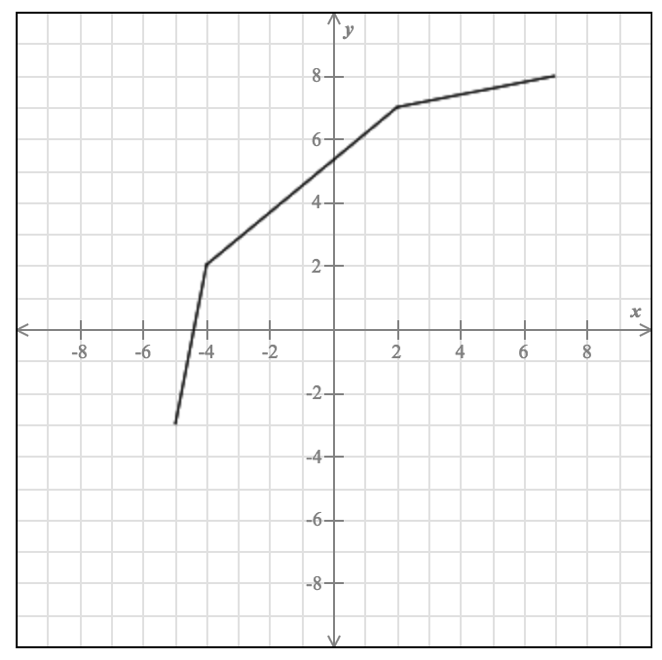
\includegraphics[width=0.5\linewidth]{1-intro3.png}
	
	
  
	
	\item Find the domain of each function:
	\[g(x)=\dfrac 4{e^x}\qquad\qquad\qquad
	 f(x)=\sqrt{1+e^x}\qquad\qquad\qquad
	 h(x)=\sqrt{1-3^x}\]
	  
	\vfill
	
	
	\item Sketch the graph of the curve $y=4e^{x-2}-1$.
	
	\vfill\newpage
	
	\item Let $\displaystyle h(x)=\frac{3x}{x-5}$. Find $h^{-1}$ and state the domain and range of $h^{-1}$ in interval notation.
	
	\vspace{200pt}
	
	\item Find the exact value of each expression.
	\begin{enumerate}
	  \item $\displaystyle \sin^{-1}\left(\frac{-\sqrt 3}2\right)$
	  
	  \vfill
	  
	  \item $\displaystyle \cos^{-1}\left(\cos\left[\frac{-\pi }6\right]\right)$
	  
	  \vfill
	  
	  \item $\displaystyle \log_5100+\log_525-2\log_52$
	  
	  \vfill
	  
	  \item $\displaystyle e^{2\ln 6}$
	  
	  \vfill
	  
	  \item $\displaystyle \sin\left(2\cos^{-1}(4x)\right)$\\
	  (\emph{Hint: use a trig identity!})
	  
	  \vfill
	  
	\end{enumerate}
\end{enumerate}


\end{document}

